\subsection{Flickering effect}

\subsubsection{Problem definition}

The time of flight technology has some limitations. Indeed, the depth value for a static object varies over time. It results in a flickering visual effect which is disturbing for a meeting room application because this variation of the depth is visible by a human eye when the point cloud of the scene is created frame after frame. This flickering effect is accentuated when several views are aligned because one view can pass in front of another and vice versa very quickly.

The following experiment has been done to quantify this variation in the depth information. A ChArUco board was placed at the place of the human subject, see figure \ref{figure:corner_detected}. The board acts as a static subject. The distance of the cameras from the board was about 1.2 meter. 120 frames (i.e. 4 seconds) were captured from each view. The position of the 24 corners in pixel was found thanks to OpenCV library. For each corner, its depth was extracted from the corresponding depth image.


\begin{figure}[H]
\centering
  \begin{subfigure}[b]{0.48 \textwidth}
    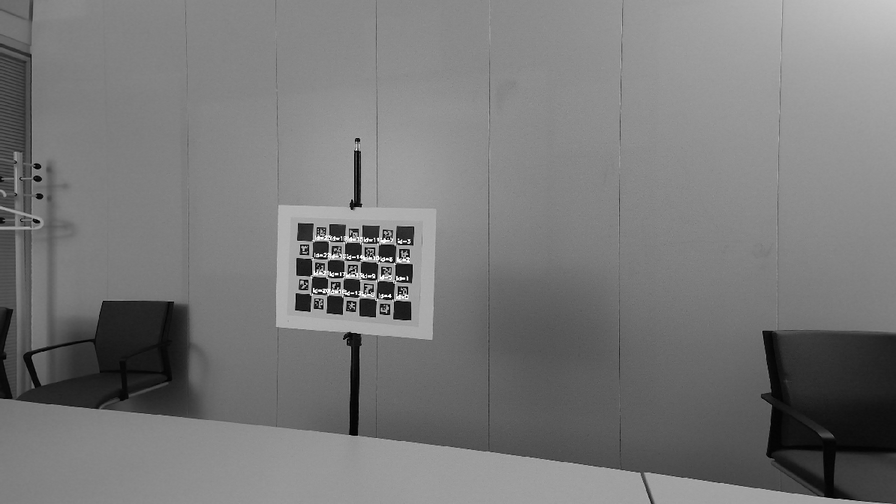
\includegraphics[width=\textwidth]{images/visual_enhancement/master_corner_detected_resized.png}
    \caption{Detection of the 24 corners from camera 1}
    \label{figure:master_corner_detected_resized}
  \end{subfigure}
  \hfill
  \begin{subfigure}[b]{0.48 \textwidth}
    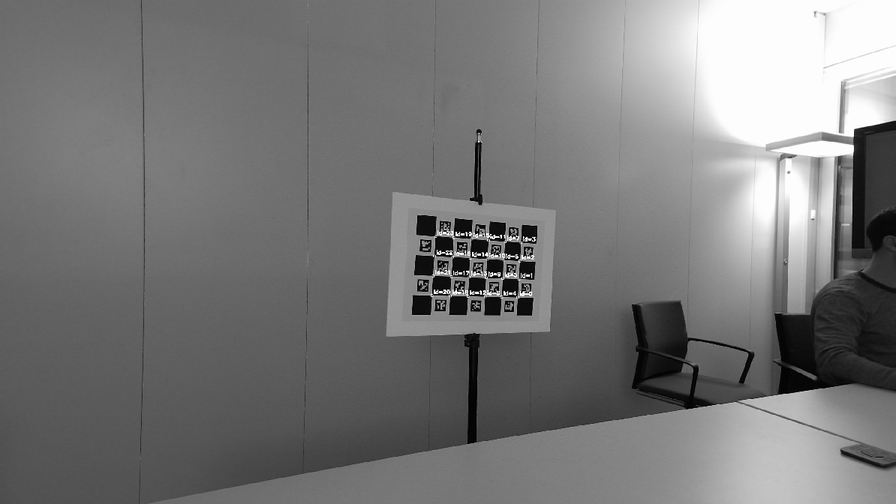
\includegraphics[width=\textwidth]{images/visual_enhancement/sub_corner_detected_resized.png}
    \caption{Detection of the 24 corners from camera 2}
    \label{figure:sub_corner_detected_resized}
  \end{subfigure}
  \caption{Detection of the 24 corners of the ChArUco board from both cameras}
  \label{figure:corner_detected}
\end{figure}

The mean of the depth of each point is subtracted to then compare them one from another. The standard deviation of the depth from camera 1 and camera 2 is respectively 3.84 mm and 3.37 mm. Figure \ref{figure:depth_curve} shows the distributions of the depth over 120 frames (i.e. 4 seconds) for these 24 points detected on the ChArUco board for both views.

\begin{figure}[H]
\centering
  \begin{subfigure}[b]{0.48 \textwidth}
    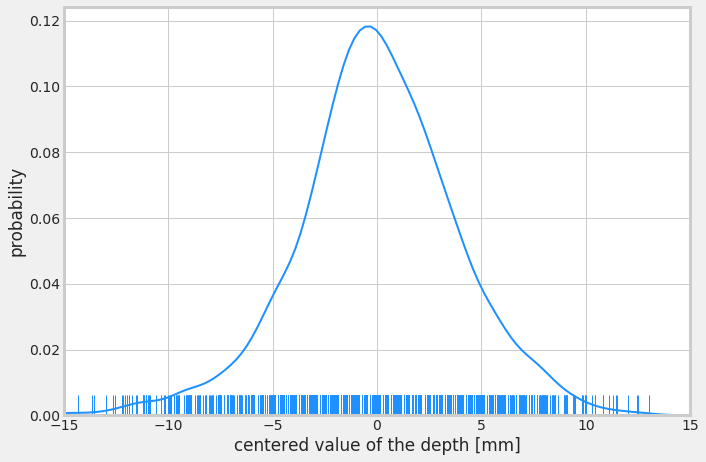
\includegraphics[width=\textwidth]{images/visual_enhancement/master_depth_curve.png}
    \caption{Distribution of the depth from camera 1}
    \label{figure:master_depth_curve}
  \end{subfigure}
  \hfill
  \begin{subfigure}[b]{0.48 \textwidth}
    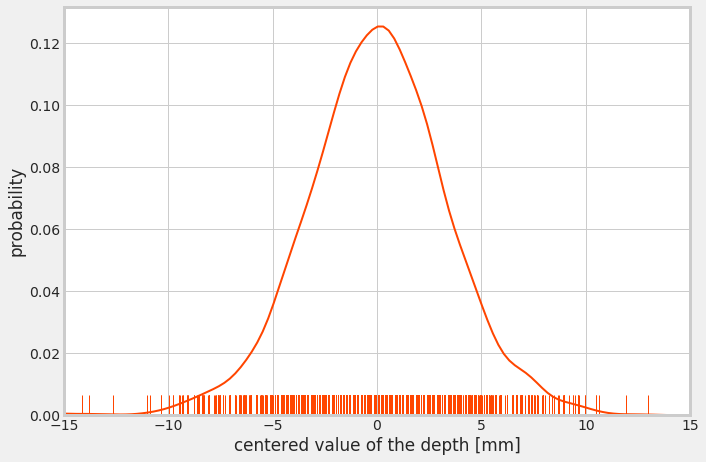
\includegraphics[width=\textwidth]{images/visual_enhancement/sub_depth_curve.png}
    \caption{Distribution of the depth from camera 2}
    \label{figure:sub_depth_curve}
  \end{subfigure}
  \caption{Probability distribution of the depth after subtracting the mean for each of the different 24 points detected on the ChArUco board}
  \label{figure:depth_curve}
\end{figure}

Figure \ref{figure:frame_serie} shows the variation of the depth over time. After analysing the variation of the depth for a static object, an implementation of a low pass filter was decided.

% Table \ref{tab:depth_stat} shows the statistics for the depth from the two different views. The difference of the minimum

% add annex of the 24 points of both views
% \begin{table}[H]
% \centering
% \begin{tabular}{c|c|c|c|c}
%  & \textbf{\begin{tabular}[c]{@{}c@{}}mean of\\ peak to peak\\ {[}mm{]}\end{tabular}} & \textbf{\begin{tabular}[c]{@{}c@{}}mean of\\ standard deviation\\ {[}mm{]}\end{tabular}} & \textbf{\begin{tabular}[c]{@{}c@{}}max of \\ peak to peak\\ {[}mm{]}\end{tabular}} & \textbf{\begin{tabular}[c]{@{}c@{}}min of\\ peak to peak\\ {[}mm{]}\end{tabular}} \\ \hline
% \textbf{view 1} & 21.25 & 3.79 & 26 & 16 \\
% \textbf{view 2} & 19.33 & 3.33 & 25 & 14
% \end{tabular}
% \caption{Statistics of the depth over the 24 points extracted from the ChArUco board. 120 frames were taken. Peak to peak is the range of values (maximum - minimum)}
% \label{tab:depth_stat}
% \end{table}


\begin{figure}[H]
\centering
  \begin{subfigure}[b]{0.48 \textwidth}
    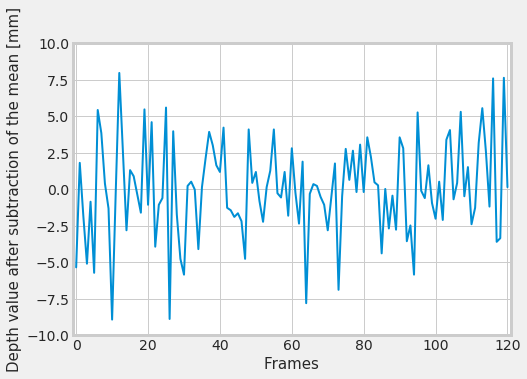
\includegraphics[width=\textwidth]{images/visual_enhancement/master_depth_frame_serie.png}
    \caption{Average centred value of the depth from camera 1}
    \label{figure:master_depth_frame_serie}
  \end{subfigure}
  \hfill
  \begin{subfigure}[b]{0.48 \textwidth}
    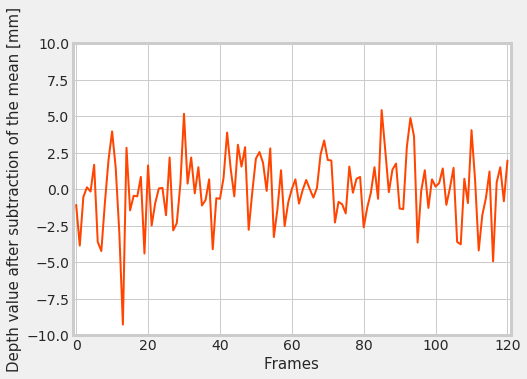
\includegraphics[width=\textwidth]{images/visual_enhancement/sub_depth_frame_serie.png}
    \caption{Average centred value of the depth from camera 2}
    \label{figure:sub_depth_frame_serie}
  \end{subfigure}
  \caption{Average value of the depth of the different 24 points detected on the ChArUco board after subtracting the mean for each}
  \label{figure:frame_serie}
\end{figure}


\subsubsection{Proposed method}

The proposed method is called "conditional moving average", see algorithm \ref{algo:conditional_moving_average}. Figure \ref{figure:flickering_backgorund_std} presents the pipeline of this approach. It takes inspiration of traditional moving average algorithm that acts as a low pass filter, see equation (\ref{equation:simple_moving_average}).

\begin{equation}
\label{equation:simple_moving_average}
    \begin{aligned}
    \bar{d}_{\mathrm{SM}} &=\frac{d_{0}+d_{-1}+\cdots+d_{-(n-1)}}{n} \\
    &=\frac{1}{n} \sum_{i=0}^{n-1} d_{-i}
    \end{aligned}
\end{equation}

where:
\begin{itemize}
    \item $n$ is the size of the window
    \item $d_i$ are the depth images
    \item $\bar{d}_{\mathrm{SM}}$ is the average over the last $n$ frames
\end{itemize}

\leavevmode\newline

\begin{figure}[H]
    \centering
    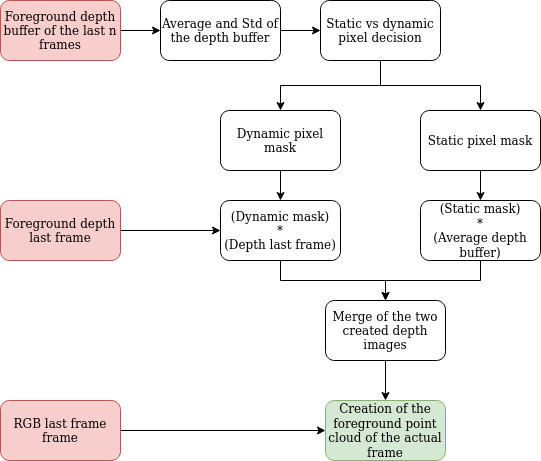
\includegraphics[width=0.65\textwidth]{images/visual_enhancement/flickering_backgorund_std.png}
    \caption{Pipeline of the conditional moving average procedure.  Input: Red boxes. Output: green box.}
    \label{figure:flickering_backgorund_std}
\end{figure}



This "conditional moving average" algorithm is applied to the depth images of both views before creating the corresponding point clouds. It distinguishes "static region" and a "dynamic region" based on a threshold. This distinction is done pixelwise. A pixel is considered as "dynamic" when the standard deviation of its depth in the buffer is above a selected threshold. The following figure \ref{figure:conditional_moving_average} illustrates the idea of the algorithm \ref{algo:conditional_moving_average}.

\begin{figure}[H]
    \centering
    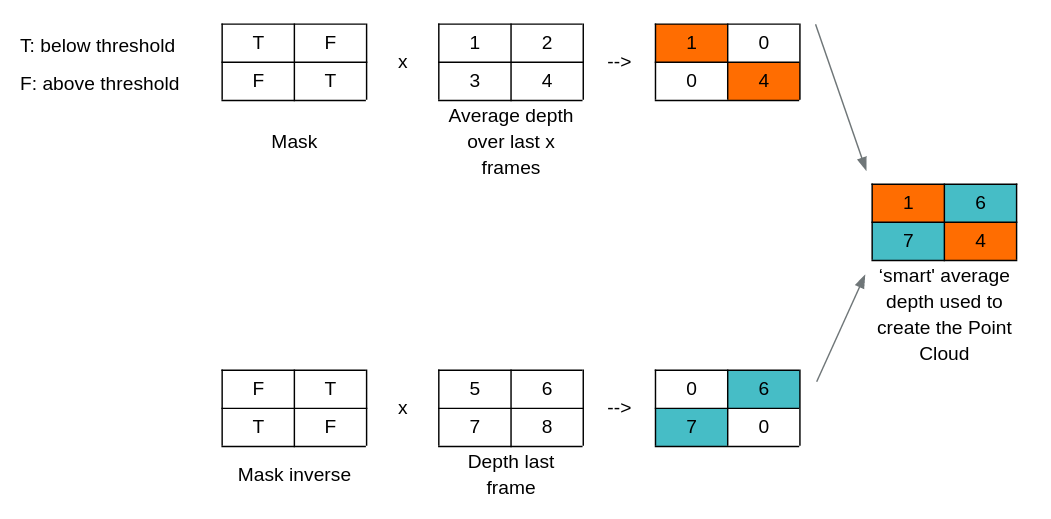
\includegraphics[width=0.65\textwidth]{images/visual_enhancement/conditional_moving_average.png}
    \caption{Pipeline of the proposed conditionnal moving average approach}
    \label{figure:conditional_moving_average}
\end{figure}

Doing this distinction between a "static region" and a "dynamic region" avoids a shadow effect visible in the case of a traditional moving average, see following section \ref{section:results_flickering}.


\begin{algorithm}
    \caption{Conditional moving average algorithm}
    \label{algo:conditional_moving_average}
    \begin{algorithmic}[1] % The number tells where the line numbering should start
        \Procedure{Conditional-Moving-Average}{$bufferDepthFrame, threshold$}
            \State $bufferAverage\gets$ pixelwise average of the last n frames of the depth buffer
            \State  $Std \gets$ pixelwise standard deviation within the buffer
            \State $mask\gets$ $Std$ < $threshold$ \Comment{True: static pixel}
            \State $averageMasked\gets$ $bufferAverage$ * $mask$
            \State $maskInverse\gets$ inverse of $maks$
            \State $lastFrameMasked\gets$ $lastFrames$ * $maskInverse$
            \State $conditionalAverage\gets$ $lastFramesMasked$ + $averageMasked$
            \newline
            \State \textbf{return} $conditionalAverage$
        \EndProcedure
    \end{algorithmic}
\end{algorithm}


% % explain the algo

% \textbf{Conditional moving average}

% t is calculated for each over the last 10 frames. It results in a more stable image. A problem occurs when the scene is dynamic. A shadow effect is visible when the subject is moving, see figure \ref{figure:shadow_effect}

% \begin{figure}[H]
%     \centering
%     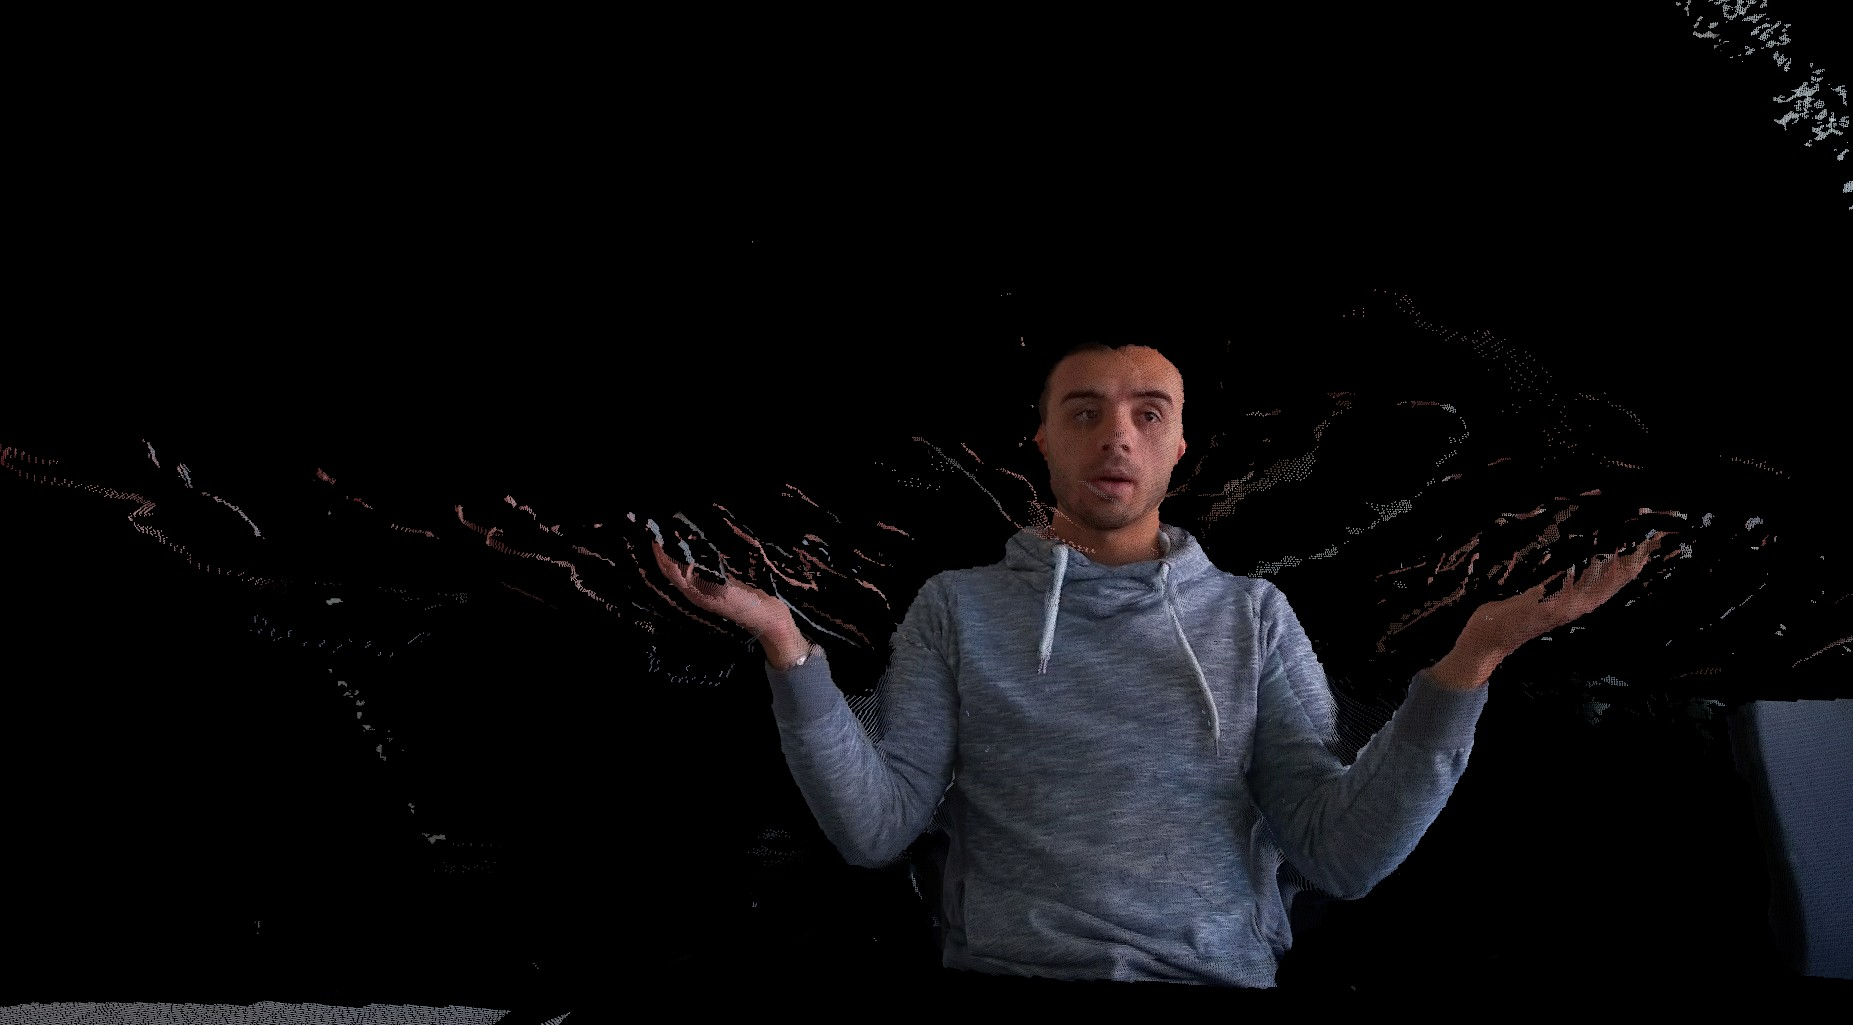
\includegraphics[width=0.65\textwidth]{images/visual_enhancement/average_5_00541.jpg}
%     \caption{Shadow effect due to the moving average of the depth images}
%     \label{figure:shadow_effect}
% \end{figure}

% The main ideas of the proposed algorithm \ref{algo:conditional_moving_average} to avoid this shadow effect are the following:
% \begin{itemize}
%     \item Take the depth average only in the ‘static’ region
%     \item Keep the current value of the depth in the ‘dynamic’ region
% \end{itemize}

% % The distinction between a "static" region and a "dynamic region" is based on a threshold. It is done pixelwise. A pixel is considered as "dynamic" when the difference between the maximum and the minimum value (peak to peak) of its depth in the buffer is above a selected threshold. The following figure illustrates this idea:

% The distinction between a "static region" and a "dynamic region" is based on a threshold. It is done pixelwise. A pixel is considered as "dynamic" when the standard deviation of its depth in the buffer is above a selected threshold. The following figure \ref{figure:conditional_moving_average} illustrates this idea:

% \begin{figure}[H]
%     \centering
%     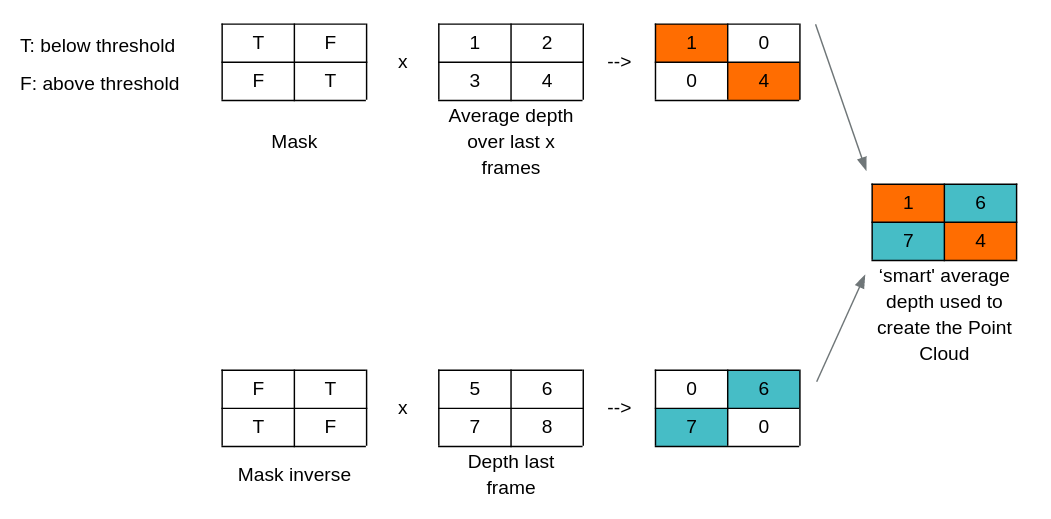
\includegraphics[width=0.65\textwidth]{images/visual_enhancement/conditional_moving_average.png}
%     \caption{Illustration of the conditional moving average for the depth with a 2x2 pixel image.}
%     \label{figure:conditional_moving_average}
% \end{figure}

% Doing this distinction between a "static region" and a "dynamic region" avoid the shadow effect and improve the quality of the rendering, see figure \ref{figure:condtional_shadow_effect}.

% \begin{figure}[H]
%     \centering
%     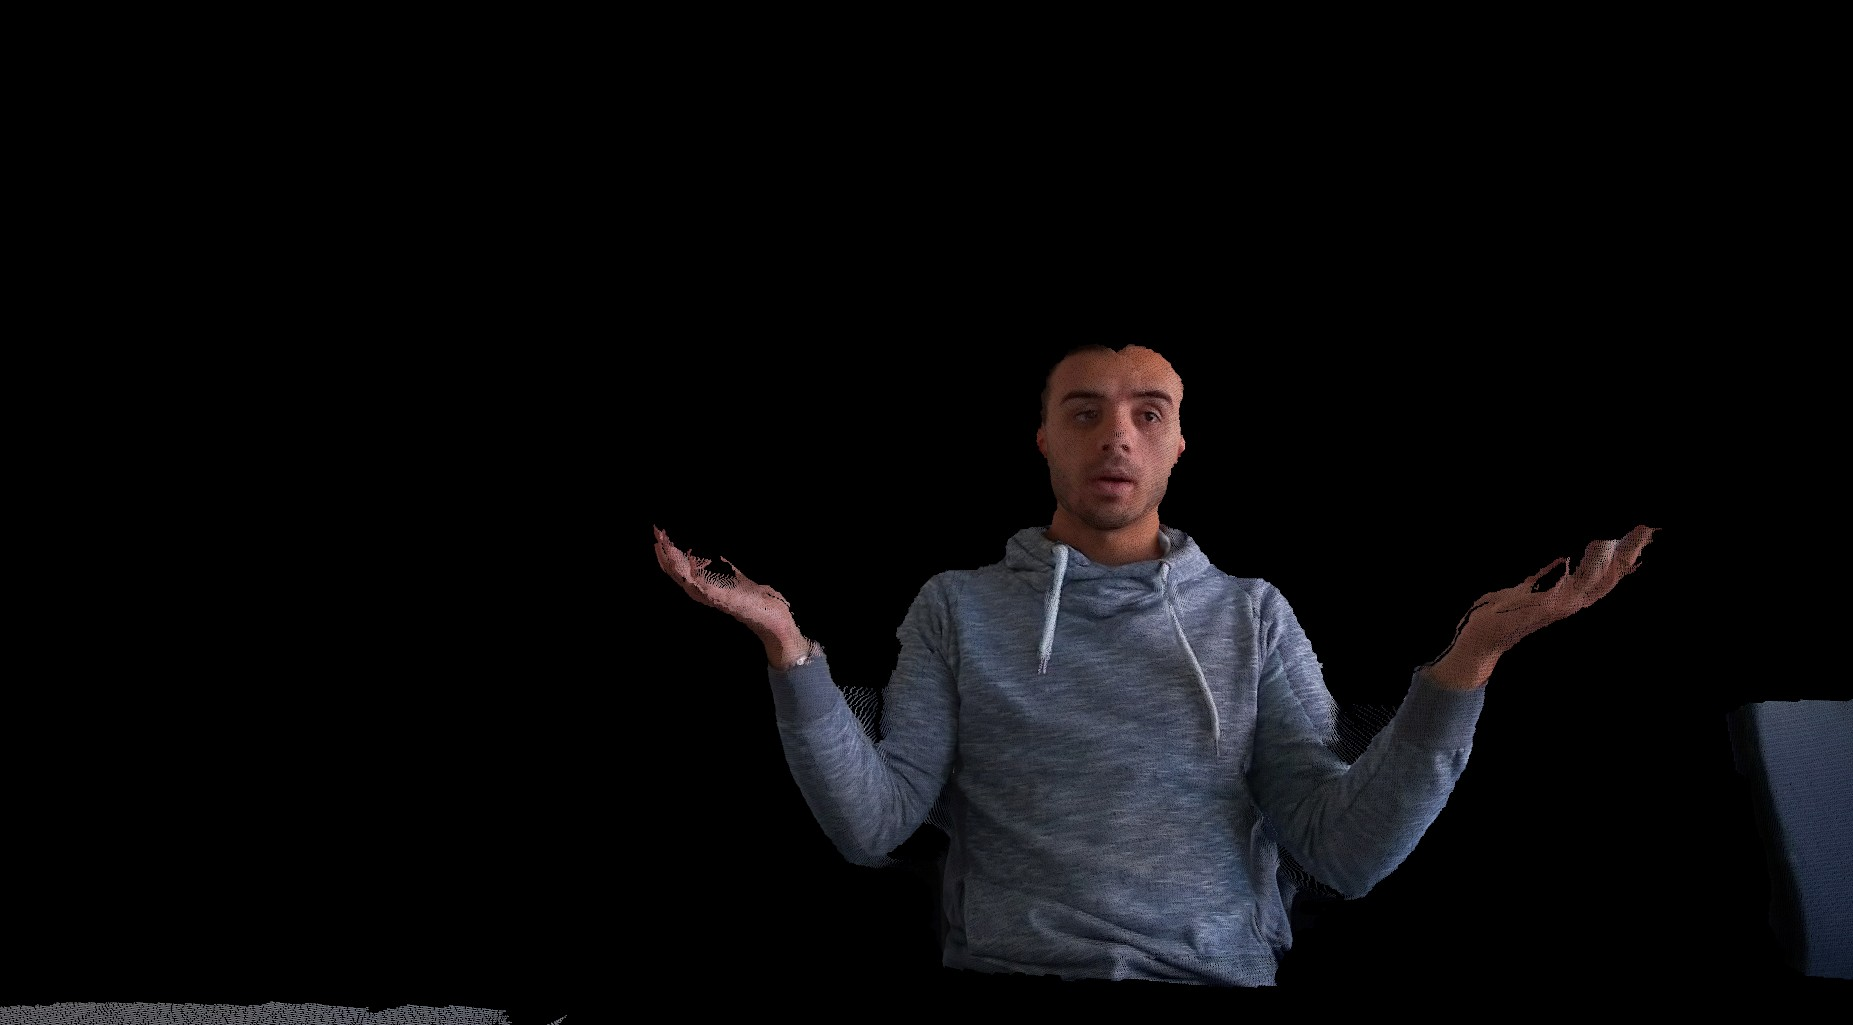
\includegraphics[width=0.65\textwidth]{images/visual_enhancement/average_5_00541_30mm.jpg}
%     \caption{Cancellation of the shadow effect thanks to the conditional moving average}
%     \label{figure:condtional_shadow_effect}
% \end{figure}




\subsubsection{Result}
\label{section:results_flickering}

Applying a moving average reduces significantly the flickering effect. Figure \ref{figure:frame_serie_moving_avarage} shows the result of applying this algorithm on the 24 corners of the board. Table \ref{tab:moving_average} shows how much the standard deviation is reduced in this ChArUco board experiment.

\begin{figure}[H]
\centering
  \begin{subfigure}[b]{0.48 \textwidth}
    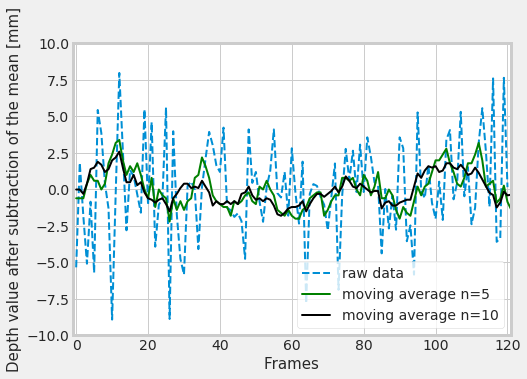
\includegraphics[width=\textwidth]{images/visual_enhancement/master_depth_frame_serie_moving_average.png}
    \caption{Average centred value of the depth from camera 1}
    \label{figure:master_depth_frame_serie_moving_average}
  \end{subfigure}
  \hfill
  \begin{subfigure}[b]{0.48 \textwidth}
    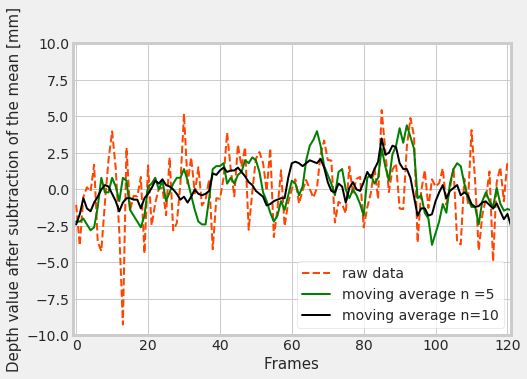
\includegraphics[width=\textwidth]{images/visual_enhancement/sub_depth_frame_serie_moving_average.png}
    \caption{Average centred value of the depth from camera 2}
    \label{figure:sub_depth_frame_serie_moving_average}
  \end{subfigure}
  \caption{Average value of the depth of the different 24 points detected on the ChArUco board after subtracting the mean for each point.}
  \label{figure:frame_serie_moving_avarage}
\end{figure}



\begin{table}[H]
\centering
\begin{tabular}{c|c|c|c}
 & \textbf{\begin{tabular}[c]{@{}c@{}}Std of the raw data\\ {[}mm{]}\end{tabular}} & \textbf{\begin{tabular}[c]{@{}c@{}}Std of the moving average\\ Window: 5 frames\\ {[}mm{]}\end{tabular}} & \textbf{\begin{tabular}[c]{@{}c@{}}Std of the moving average\\ Window: 10 frames\\ {[}mm{]}\end{tabular}} \\ \hline
\textbf{view 1} & 3.79 & 1.57 & 1.09 \\
\textbf{view 2} & 3.33 & 1.50 & 1.04
\end{tabular}
\caption{Statistics of the depth over the 24 points extracted from the ChArUco board. 120 frames were taken.}
\label{tab:moving_average}
\end{table}

Visually this decrease in the standard deviation is noticeable and improves the experience.  The proposed conditional version of the moving average algorithm avoids the shadow effect visible when no distinction between "static" vs "dynamic" pixel is done, see figure \ref{figure:master_depth_frame_serie_moving_average} This shadow effect is a problem handled by the proposed approach, see figure \ref{figure:average_5_00541_30mm}.

% \begin{figure}[H]
%     \centering
%     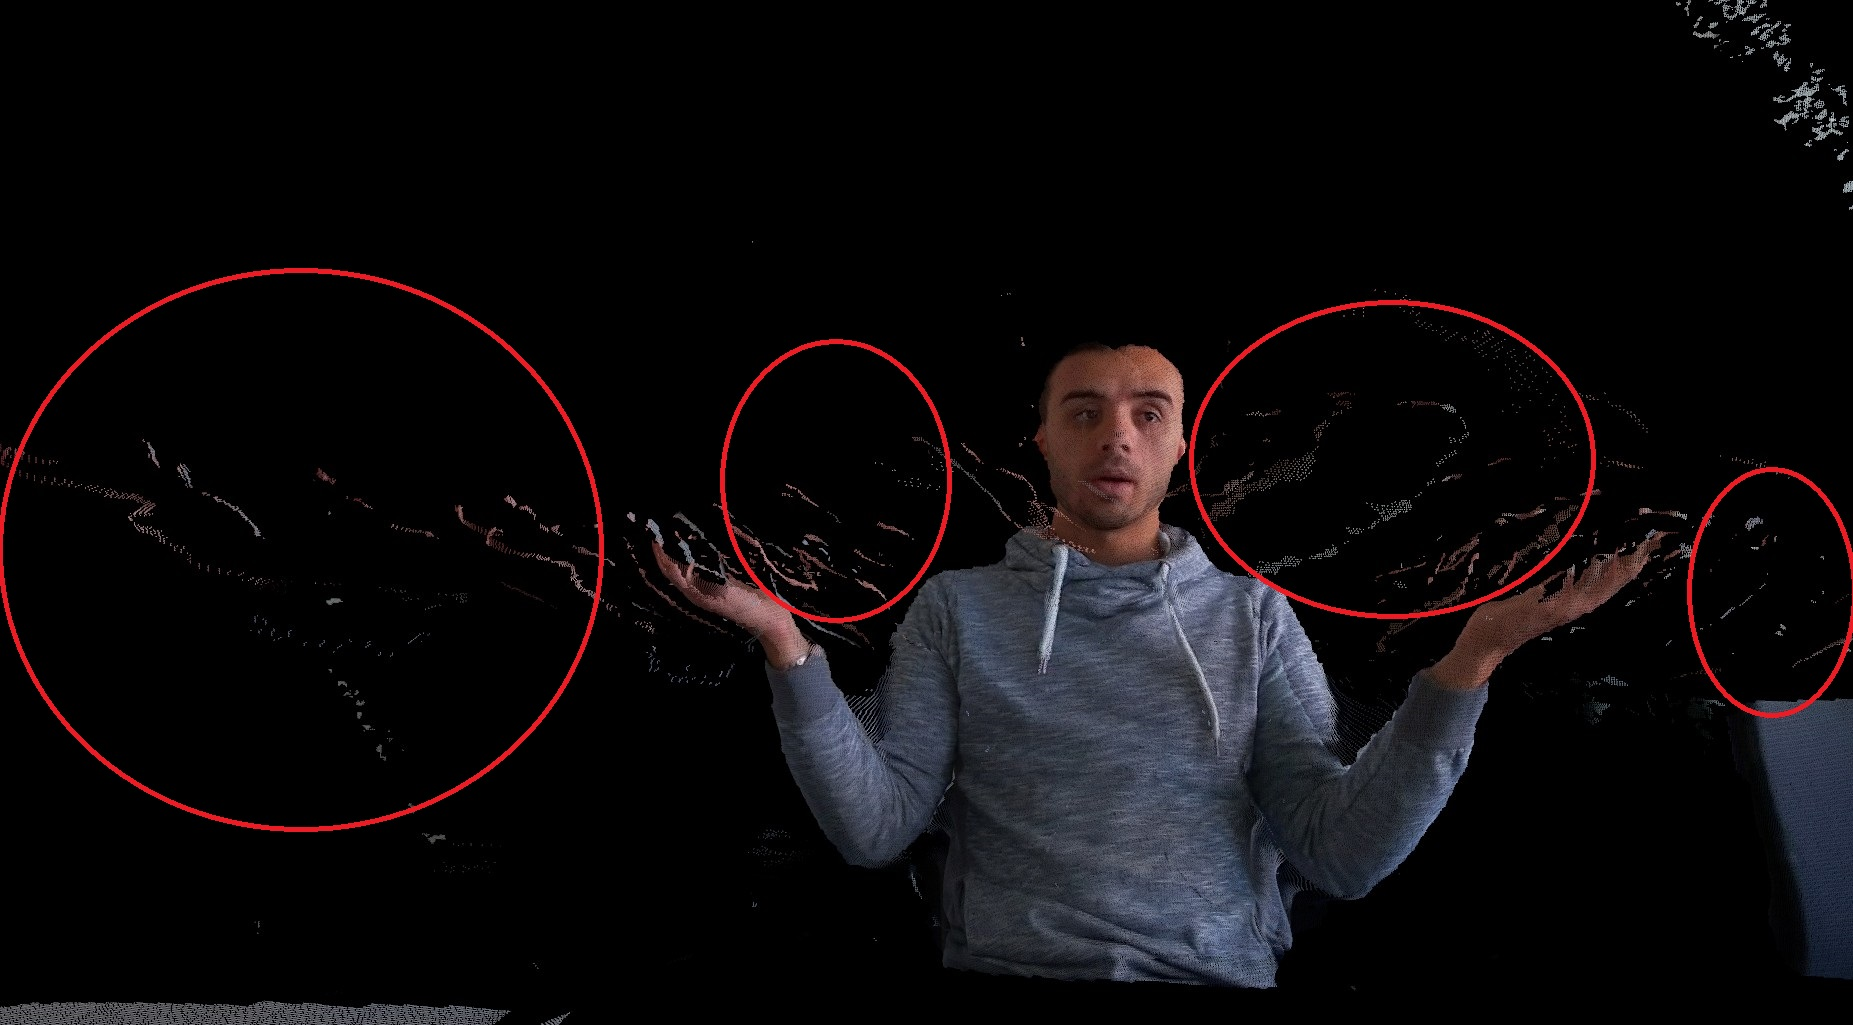
\includegraphics[width=0.65\textwidth]{images/visual_enhancement/average_5_00541_red.jpg}
%     \caption{Shadow effect due to the moving average of the depth images}
%     \label{figure:average_5_00541_red}
% \end{figure}



\begin{figure}[H]
\centering
  \begin{subfigure}[b]{0.65 \textwidth}
    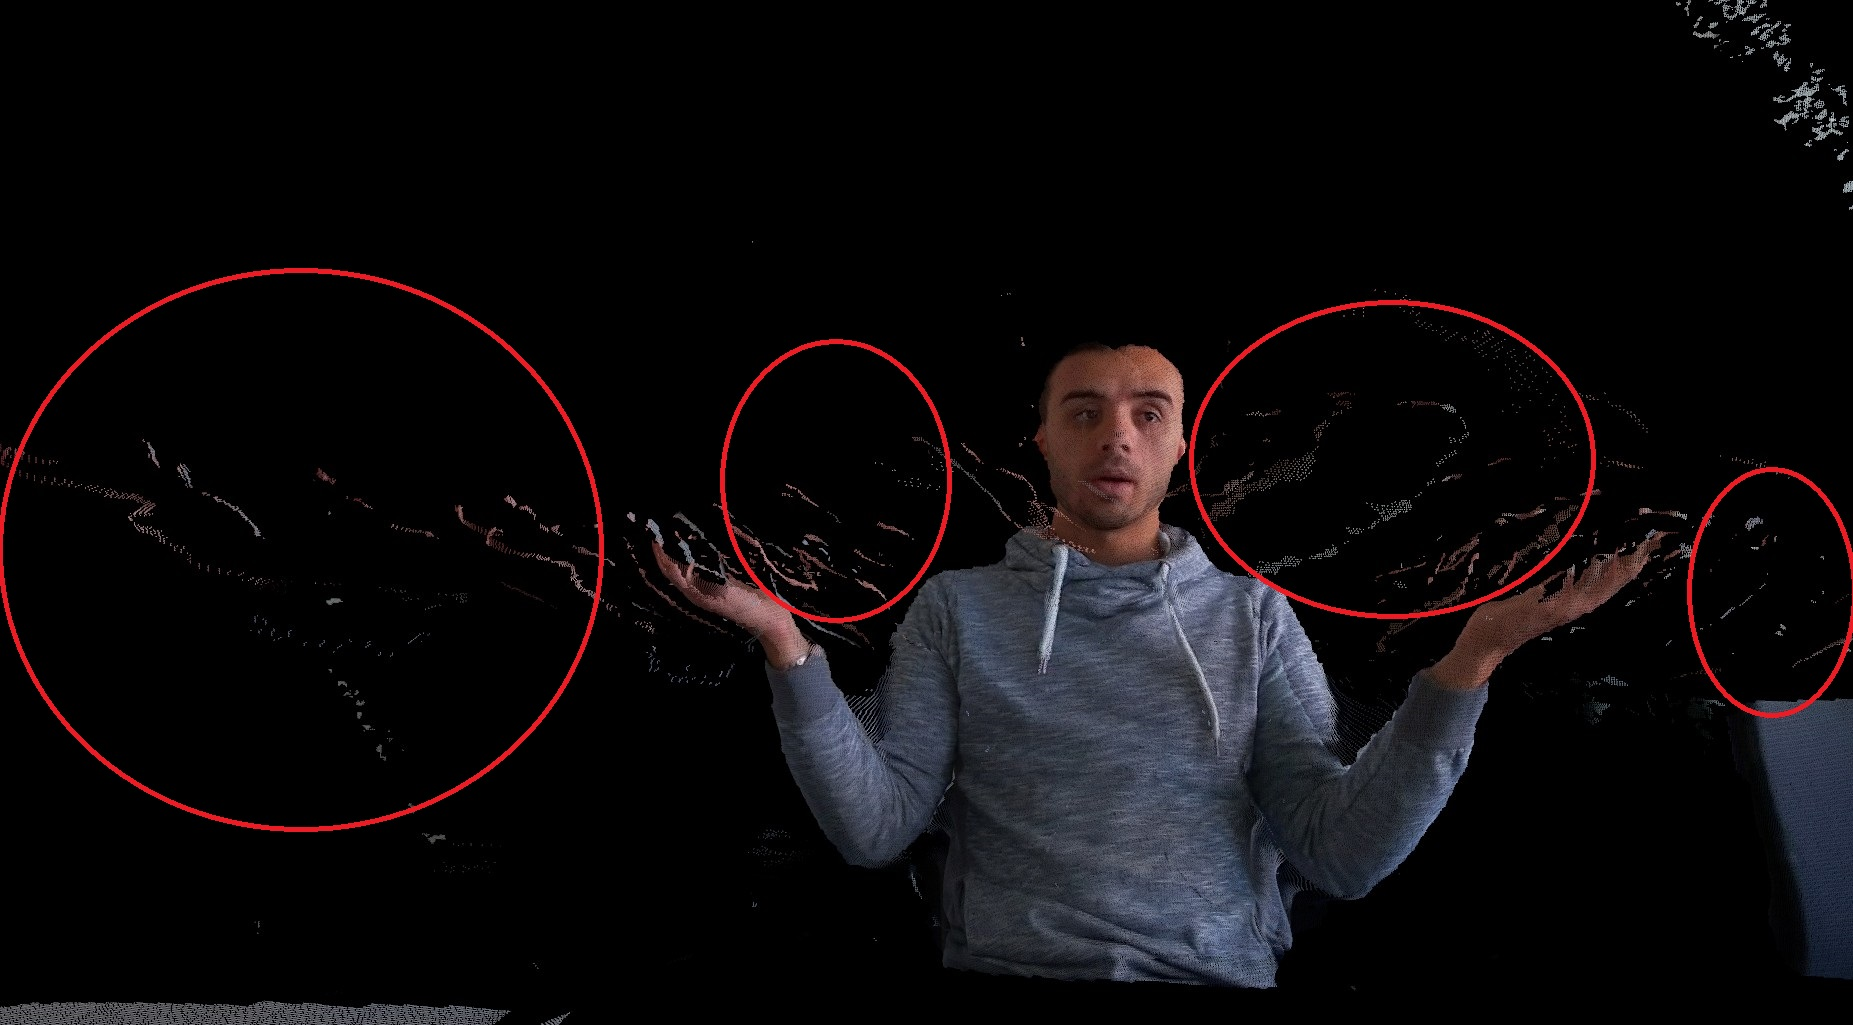
\includegraphics[width=\textwidth]{images/visual_enhancement/average_5_00541_red.jpg}
    \caption{Shadow effect due to the traditional moving average of the depth images}
    \label{figure:master_depth_frame_serie_moving_average}
  \end{subfigure}
  \hfill
  \begin{subfigure}[b]{0.65 \textwidth}
    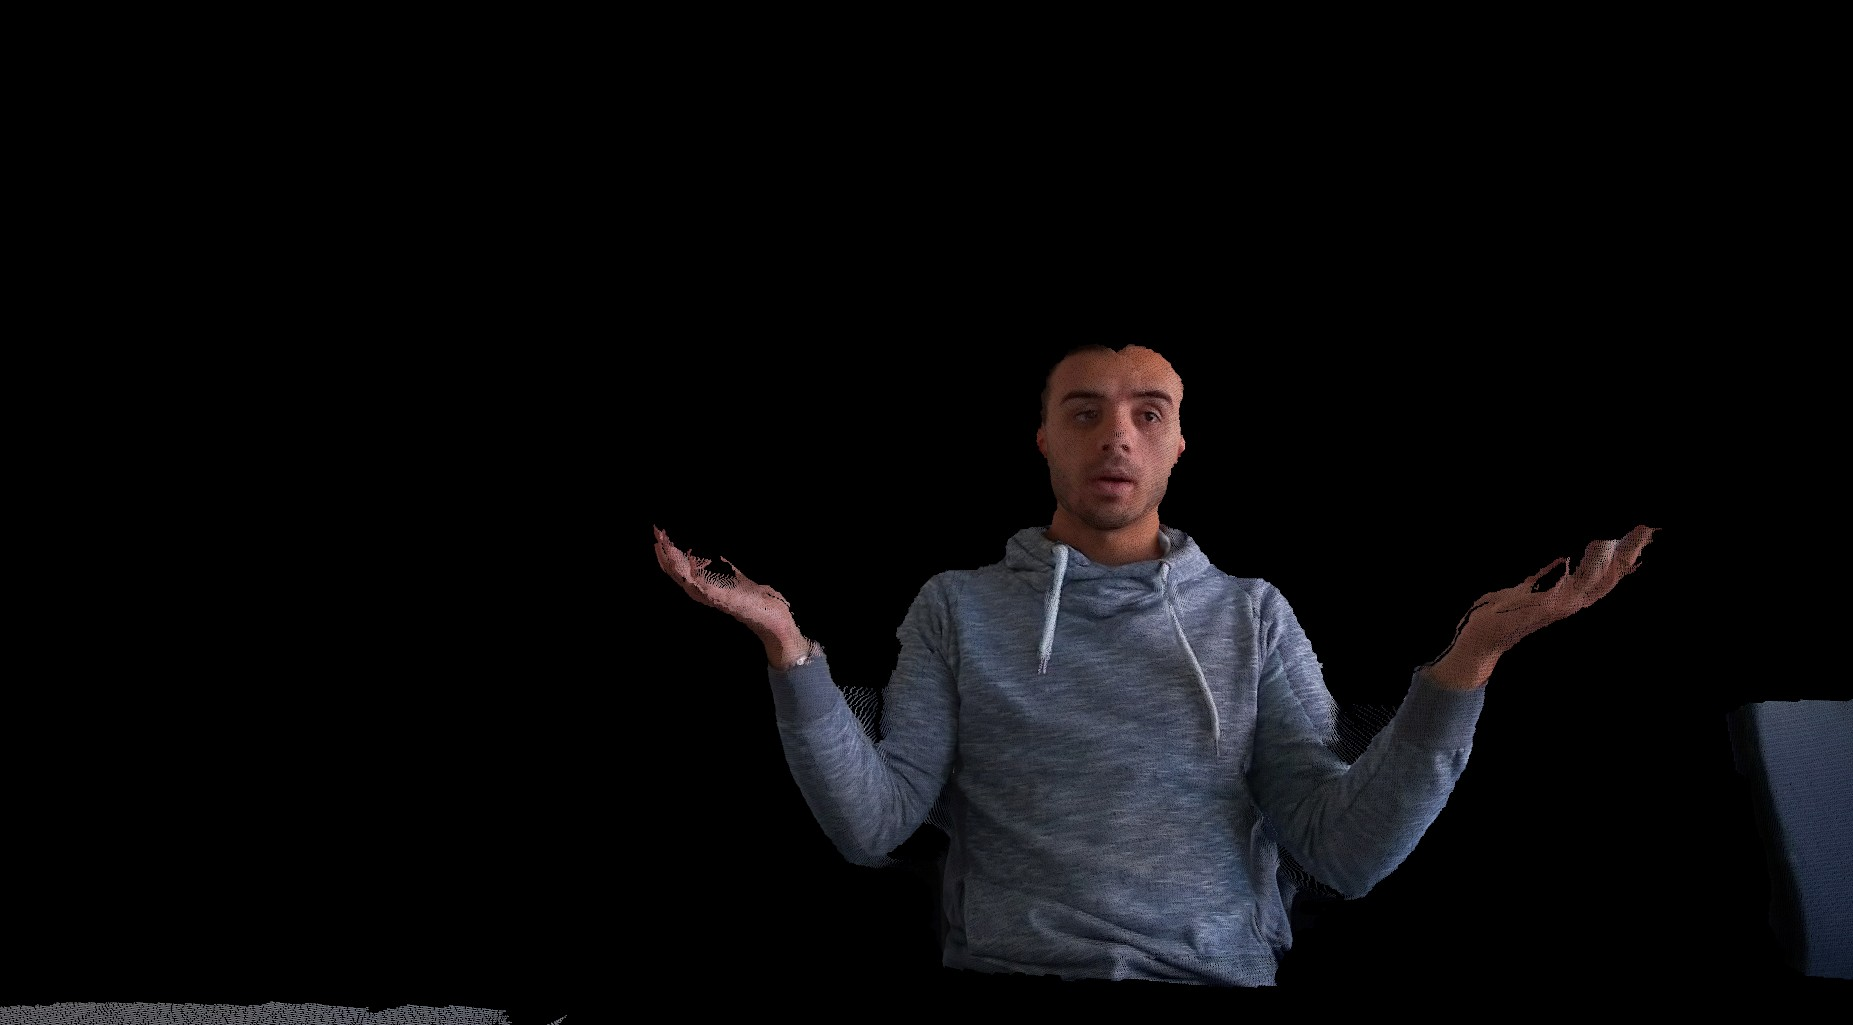
\includegraphics[width=\textwidth]{images/visual_enhancement/average_5_00541_30mm.jpg}
    \caption{Cancellation of the shadow effect due thanks to the conditional moving average}
    \label{figure:average_5_00541_30mm}
  \end{subfigure}
  \caption{Comparison of the two different moving average algorithm}
  \label{figure:frame_serie_moving_avarage}
\end{figure}

However, the conditional moving average algorithm has some limitations. Increasing the window of this moving average algorithm decreases the standard deviation but it also increases the delay in the "dynamic region" of the scene. A trade-off was found empirically and the window $n$ was fixed at 5 frames.

Another limitation appears when the point of view is a virtual. Because the decision between a "dynamic region" versus a "static region" is based on a threshold, the separation between theses regions is visible when the "dynamic region" is moving "too fast". A step appears in the 3D space. Figure \ref{figure:limitation_00497_5_50_red} shows an example of this undesirable effect. Some black lines are visible. They are in fact the colour of the background.

\begin{figure}[H]
    \centering
    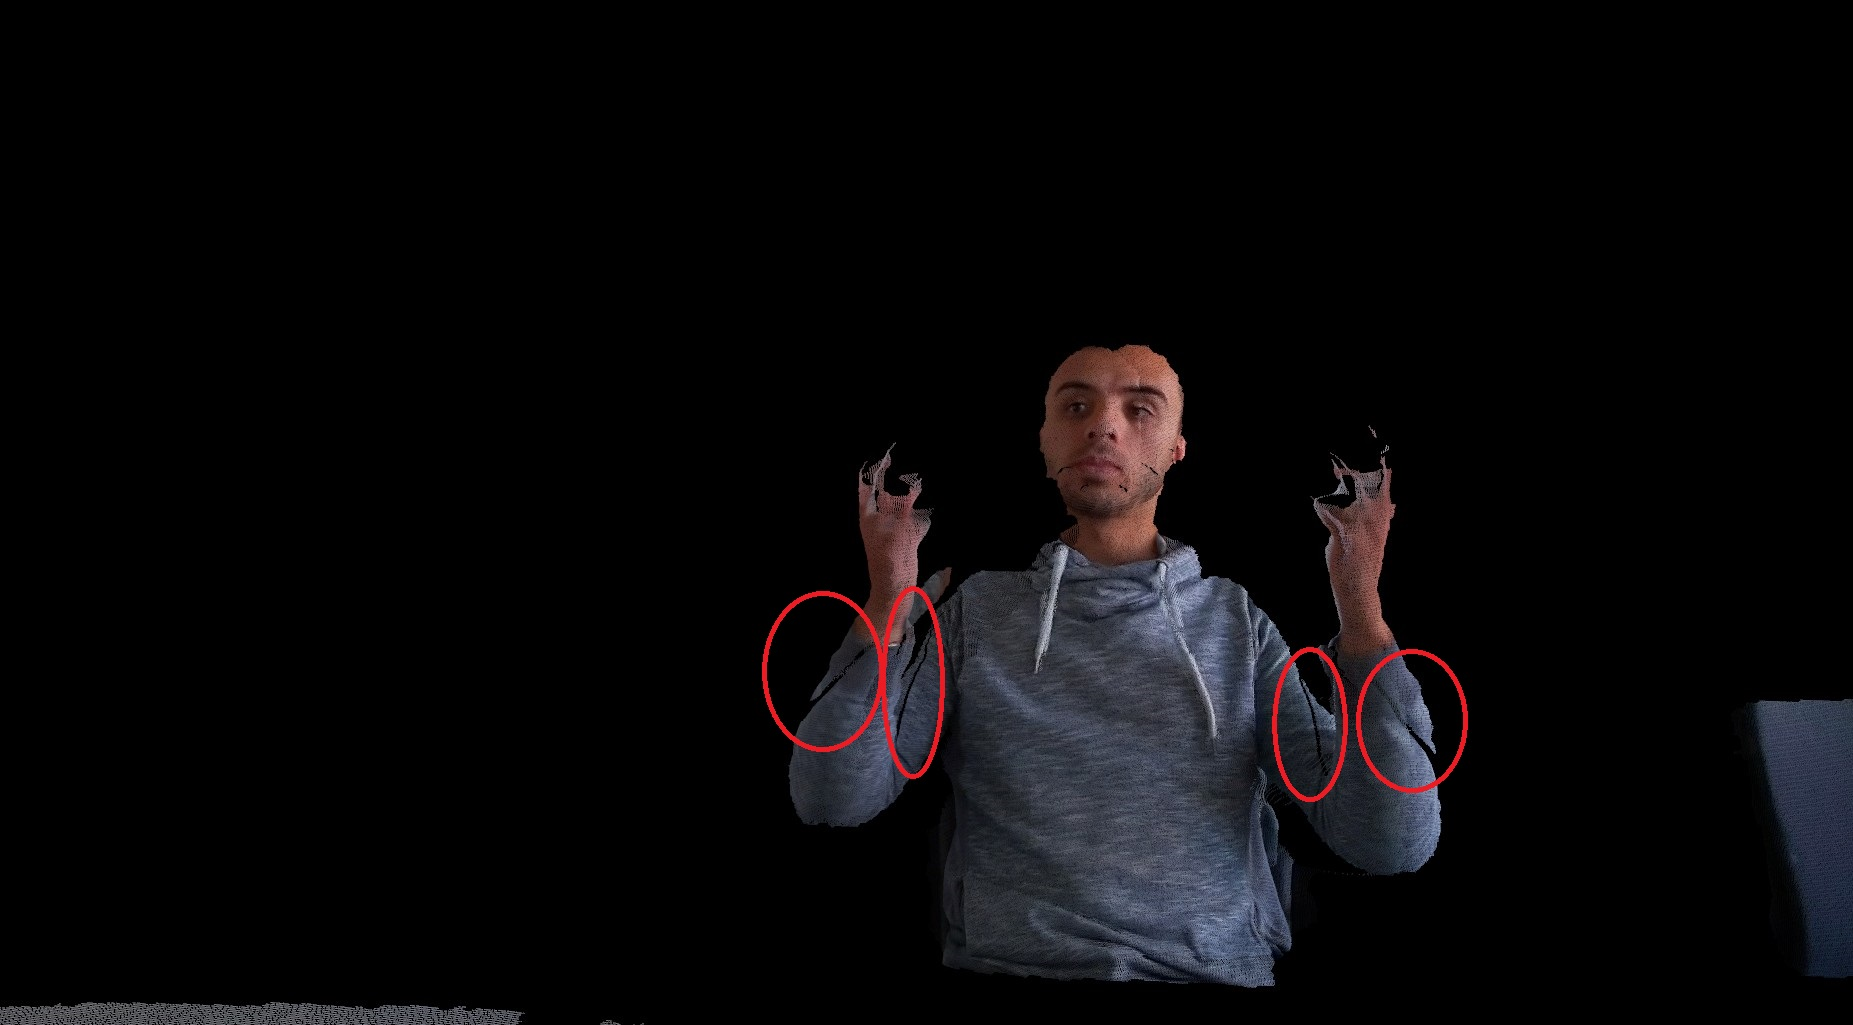
\includegraphics[width=0.65\textwidth]{images/visual_enhancement/limitation_00497_5_50_red.jpg}
    \caption{Limitation of the conditional moving average. Lines appear in the "dynamic region". These lines are visible when the point of view is virtual.}
    \label{figure:limitation_00497_5_50_red}
\end{figure}

The following figure is a zoom on the face. The subject was moving fast. Therefore, the decision between "dynamic" versus "static" region based on a threshold is clearly visible when the point of view is virtual.

\begin{figure}[H]
    \centering
    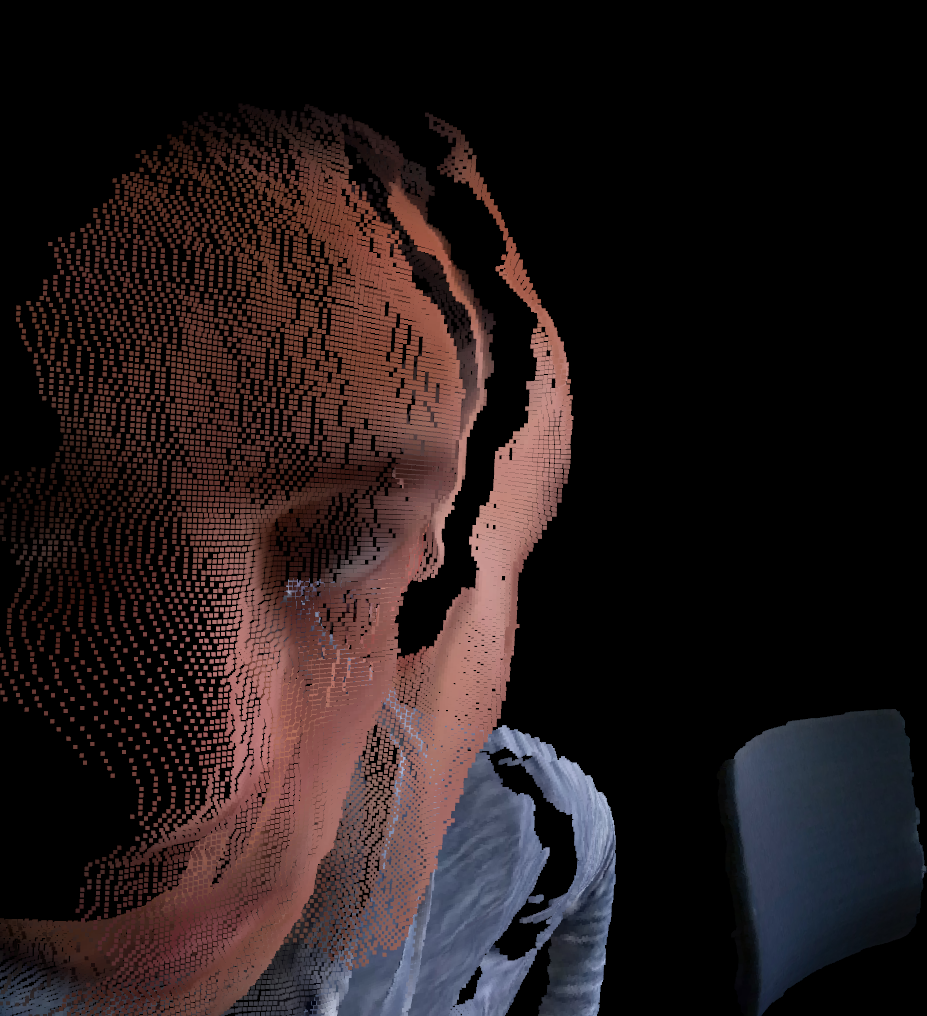
\includegraphics[width=0.35\textwidth]{images/visual_enhancement/edge/zoom_lines.png}
    \caption{Zoom on the limitation due to the threshold. based decision between "static" and "dynamic" region}
    \label{figure:zoom_lines}
\end{figure}

\subsubsection{Discussion}

The conditional moving average algorithm developed to tackle the limitation of the hardware is efficient. It reduces visually the flickering effect significantly which was the objective of this solution. However, this flickering effect is still visible even if it is reduced. Intuitively, increasing the size of the moving average should improve the rendering. But is it not the case. It indeed limits the flickering effect but another undesirable effect becomes visible. Latency in the "static region" appears if the size of the window is too high (i.e. above 15-20 frames). A window centred conditional moving average was tried as well. The visual impact of this non-causal filter was not better than the actual one. Instead of average, median was also tried. The visual impact was not better either.

Another algorithm should be investigated to have a continuity between the "dynamic" and "static" region, especially when the point a view is a virtual one. However, for the rest of this project, the conditional moving algorithm \ref{algo:conditional_moving_average} is used.
